\documentclass[10pt]{article}
\usepackage[margin=1in]{geometry}
\usepackage{cite}
\usepackage{amsmath}
\usepackage{url}
\usepackage{graphicx}

\title{Milestone for MAUL: Machine Agent User Learning\footnote{Some unscrambling necessary.} }
\author{Robert Holley and Daniel Rosenfeld}
\date{11/12/2010} 


\begin{document}
\maketitle
\begin{abstract}
We describe implementation of a classifier for User-Agent strings using Support Vector Machines.  The best Kernel is found to be the linear kernel, even when more complicated string based kernels, such as the edit distance kernel and the subsequence kernel, are employed.  A robust tokenization scheme is employed which dramatically speeds up the calculation for the edit string and subsequence Kernels by shortening the effective string length. 
\end{abstract}


\section{Introduction}
A User-Agent string is an HTTP header sent along with a request for a web page, often but not always by a web browser.\cite{httprfc} The intent is to inform the server
of the capabilities of the software being used by the client. The User-Agent is
one of the most important signals to differentiate a desktop browser from a
mobile device or an automatic crawl. In addition gathering statistics on them
provides insights on changes in browser, operating system and device usage. They
are also frequently misused, in e.g. cloaking a web site to make it look
different to a search engine crawl.

User-Agent strings can contain loosely-structured tokens on engine, browser,
version, build date, etc. but their format was never strictly standardized.\cite{httprfc}
As the number of web-access devices increases, especially with new-generation
mobile devices and browsers, the numbers of different User-Agent strings is
rapidly growing and diversifying. Extensions and plugins can often mutate
User-Agent strings in unpredictable ways (insert, splitting, duplicating, and
re-ordering tokens). Firefox 4 and Internet Explorer 9 will soon ship with
completely reformatted strings. Some mobile operators have begun introducing
custom HTTP headers to extend the traditional role of the User-Agent.\cite{mobile} Web spiders and crawlers are also an important and unpredictable contributing factor.
An overview of the development and mutation of User-Agent strings is given in,\cite{history} while \cite{uatracker} is a public list of over 50000 currently unique strings.

For over a decade, those interested in tracking the proliferation of the web have collected User-Agent strings and built classifiers for them.  One of the first such entities was Microsoft, who included a recognition engine (browscap.dll) and a pattern file (browscap.ini) with its early web servers.\cite{bcp}  The Browser Capabilities Project (BCP) has kept these files up to date for the web development community, despite Microsoft's abandonment for more sophisticated (and proprietary) methods.\cite{bcp}  However, the maintenance of the project requires human parsing of new User-Agent strings every week and subsequent updating of the recognition engine and pattern file (BCP reports that they receive several dozen new User-Agent strings per week).  Gary Keith, the proprietor of BCP, has an automatic script run every Sunday morning, the output of which he parses in the afternoon and updates his file of highly structured regular expression searches.  A more recent effort, Browserscope (which started as UAProfiler), took a similar approach, using a regular expression based parsing engine to identify specific browsers (browsers only). \cite{souders}  The parsing engine required regular updates to remain up to date with new User-Agent strings.  In 2009, the author of UAProfiler (Steve Souders) reported finding 20 new User-Agent strings {\it per day}, which he examined every day at 7 am over morning coffee. \cite{souders2}  Other efforts such as those by user-agent-string.info and useragentstring.com, also use brittle parsing rules and curated data just like Browserscope and BCP.  \cite{uas.info,uas.com}  Other efforts to categorize User-Agent strings include entire communities such as agentarius.net, which has created a structure database of over 200,000 User-Agent strings.   

Our machine learning approach to User-Agent string parsing could provide partially automated parsing even on new User-Agent strings, absolving the need for a human to keep User-Agent parsers up to date.  Although we are quite sure Gary and Steve will continue updating their parsers each Sunday and over morning coffee, perhaps some day in the future this will not be necessary.

\section{Computational Approach}
\subsection{Data}
We have assembled an annotated dataset consisting of 53,829 User-Agent strings.  The strings were acquired from a variety of sources (user-agents.org: 2463 strings, ua-tracker.com: 50,482 strings, user-agent-string.info: 1460 strings; 53,829 total excluding duplicates.).\cite{ua.org,uatracker,uas.info}  The annotation consists of agent type (Browser, Bot), agent family (Firefox, googlebot, etc.), family version, OS (Windows, Linux, etc.), and OS version.  The annotation was performed by using two common parsing engines (UASparser\cite{uas.info} and uaParser (formerly Browserscope, formerly UA Profiler)\cite{uaParser} )) and merging the result.  Since UASparser returns the most information (a Python dictionary with User-Agent Type, Family, and OS) it is used as the primary source of information where uaParser is used to generate version information for Browsers.  uaParser is primarily geared toward parsing Browsers and therefore is not useful for Bots and the other types of entities on the web.   This approach was taken due to the lack of availability of annotated sources.  Some of the annotated User-Agent strings were curated by hand due to the failure of the parsers.  The data were parsed and annotated using a series of python scripts and python versions of the afore-mentioned parsers.  
\subsection{Data Processing}
The data generated by the above methods were additionally processed to reduce and standardize the number of classes.  Specifically, the OS information was parsed to collapse all versions of Windows, Linux and Mac OS into only three OS's and move all other OS information into the OS version field.  All special versions/modes/builds of specific Browsers were collapsed into their respective families.  All Validators and Bots were given the Type field "Robot" since Validators are also non-human web crawler applications.  The dataset is stored in both a flatfile format which allows for facile reading and editing by a human and a SQLlite database for querying for classifier codes.  
%tokenization in this section, and data pipeline
% - some testing of tokenization, i.e. addition of @, + , &
% tokenization figure
The User-Agent strings were tokenized in order to build feature vectors and also speed up the implementation of the non-vector based string Kernels we used to classify the strings.  Tokenization is an atomistic deconstruction of each User-Agent string at arbitrarily chosen break characters (See Figure 1).  The tokenization scheme used in our classifiers was to break apart the string at any instance of {\bf \textbackslash / [].,;}.  Other break characters were also attempted, such as '@' and '&', however little improvement was made.  

The tokens were further coalesced to increase the robustness of the classifier.  Instead of having a unique token for every number, all numbers of the same length were represented by a single token.  Further coalescing was performed so that instances of 'http' and '+http' were represented by a single token.      

\begin{figure}
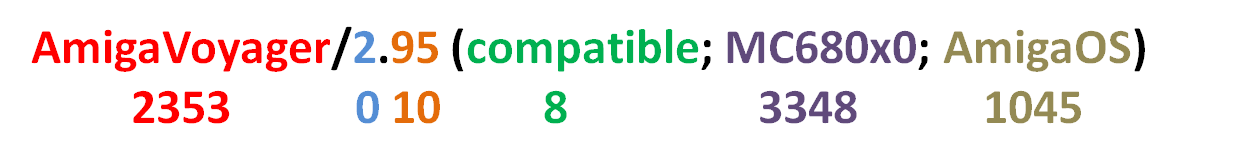
\includegraphics[width=6in]{token_figure.png}
\caption{Example of the tokenization process.  Notice that the string is deconstructed at any instance of one of the following characters: {\bf \textbackslash /[].,;}  .}
\end{figure}


\subsection{Learning Implementation}
\subsection{Learning}
% few sentences on SVM, overfitting protection
% figure on decision tree
Generally, given a new User-Agent string, our goal is to guess whether the string is from a bot, or a browser (or one of several other types).  If the string is from a browser, we will also want to guess the browser type (family) and OS type.    Our goal is to build several classifiers using different techniques in order to find the most robust for classifying User-Agent strings.  For performing SVM training and prediction we use the LIBSVM library.\cite{libsvm}  LIBSVM is accessed through a python interface to a dynamically linked library. 

Our first approach has been to use a Gaussian string edit distance kernel with an SVM.   The Kernel function is given by Eq. 1 below,
\begin{equation}
K(x,z) = \exp \left[ - \gamma \operatorname{LD} (x,z) \right]
\end{equation}
where $\operatorname{LD}(x,z)$ is the Levenshtein Edit Distance between two strings $x$ and $z$.  Using this approach an accuracy of 97\% has already been achieved using only a subset of our data (code optimization is still underway, a confusion matrix approach to error analysis is planned but not yet completed).   Given that a string is classified as a browser we then plan to attempt to fully classify it into a family and OS type using a similar edit string distance based approach.
Our second approach relies on using a recursively calculated subsequence kernel.\cite{subseqkernel}  This Kernel looks for all sub-sequences shared by two strings.  The contribution to the kernel of a shared sub-string is damped by an exponential factor related to its length in both strings.  The Kernel is mathematically described  in the above reference.  This Kernel will be used with the raw string data of the User-Agent strings, but we will also use this Kernel on a tokenized version of the User-Agent strings.  Since many User-Agent strings of similar types differ in a re-ordering of tokens, we will build a dictionary of tokens and create a new string in the space of these tokens.  
% add subsequence definition
% - additions to subsequence kernel
% 	- lookup table for lambdas
%    - generic template for any type
%   - explain why this is necessary, i.e. subsequence is extremeley slow w/o tokenization 
% - edit kernel tokenization
% discuss framework 
% 	- SQLlite
% 	- other aspects of framework

% Results
% - Kernel competition
%  	- results table
% - cases where classification can beat traditional parsing
% - ordering as a confounding factor
% - cross validation for parameter tuning
% -  

% Extensions
% - could CV on tokenization scheme
% - better token coalescence 
% - after classifying, could run a brittle parse 
% - bigger data sets are out there 
% - mozilla possible continuation
% - edit distance for nearest token


The main scope of our project consists of implementing the above SVM based approaches.  However, we will also compare the above string Kernel based approaches to feature based approaches.  Possible features are sub-strings of length k, or the presence of a particular token.  Features will be selected by scoring or backward selection.  Linear Kernel and higher order Kernel based SVMs will be used in the space of these features to classify the User-Agent strings.  The results will be compared to the string based approaches.  We also plan to use a dictionary based approach with Naive Bayes (due to its simplicity) as a method of determining a baseline performance that our more complicated efforts can be measured against.  



\bibliography{references}
\bibliographystyle{plain}
\end{document}